\chapterA{Diseño algorítmico}
\section{Introducción}
\begin{figure}[H]
	\centering
	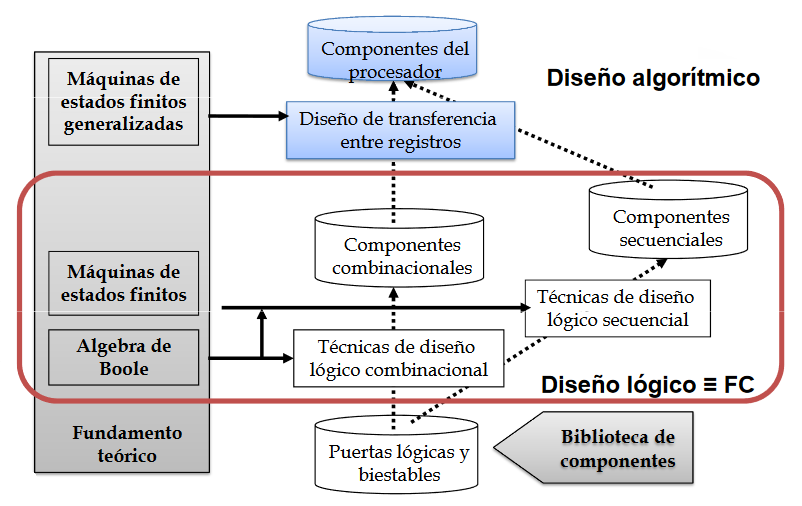
\includegraphics[width=\textwidth]{images/Tema_4/Flujo_Diseno.PNG}
	\caption{Flujo de diseño}
\end{figure}
\section{Máquinas de estados: repaso}
\subsection{Máquinas de estados finitos (FSM)}
\textbf{Mealy:} un cambio en la entrada en cualquier instante influye inmediatamente  en la salida.

\begin{multicols}{2}
	\[
		Z\left(t\right) = H\left(X\left(t\right), S\left(t\right)\right)
	\]
	\[
		S\left(t+1\right)= G\left(X\left(t\right), S\left(t\right)\right)
	\]
	\vfill
	\null
	\begin{figure}[H]
		\centering
		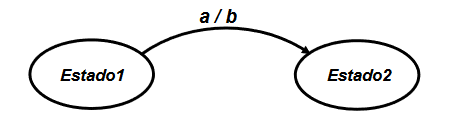
\includegraphics[width=0.3\textwidth]{images/Tema_4/Mealy.PNG}
		\caption{Ejemplo estados Mealy}
	\end{figure}
\end{multicols}

\textbf{Moore:} sólo el cambio del estado influye en la salida

\begin{multicols}{2}
	\[
		Z\left(t\right) = H\left(S\left(t\right)\right)
	\]
	\[
		S\left(t+1\right)= G\left(X\left(t\right), S\left(t\right)\right)
	\]
	\vfill
	\null
	\begin{figure}[H]
		\centering
		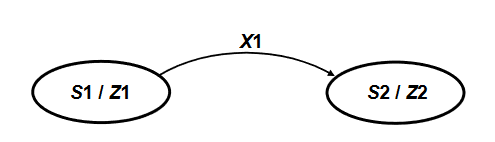
\includegraphics[width=0.3\textwidth]{images/Tema_4/Moore.PNG}
		\caption{Ejemplo estados Moore}
	\end{figure}
\end{multicols}

\subsection{Funcionamiento síncrono}
La hipótesis de funcionamiento síncrono de los sistemas secuenciales supone que:
\begin{itemize}
	\item El estado sólo cambia cada vez que el ciclo de reloj y el cambio es simultáneo en todos los bits del cambio de estado.
	\item Tras un cambio de estado, las entradas de los bits del registro de estado tienen tiempo para alcanzar un valor estable antes del siguiente cambio de estado.
\end{itemize}
\section{Elementos de memoria: repaso}
Cuando estamos diseñando un sistema secuencial uno de los elementos \gls{hw} más importantes son los elementos de almacenamiento:
\begin{itemize}
	\item Almacenan el estado actual del sistema (máquina de control)
	\item Almacenan valores intermedios (registros de datos)
\end{itemize}

El elemento de memoria más sencillo es el \textbf{biestable}. Se denomina biestable porque presenta dos únicos estados estables: Salida 0 o Salida 1. Sirve para almacenar un bit de información.
\subsection{Tipos de biestables}

\begin{multicols}{2}
	Según su comportamiento lógico:
	\begin{itemize}
		\item S-R
		\item D
		\item J-K
		\item T
	\end{itemize}
	\vfill
	\null
	Según su comportamiento temporal:
	\begin{itemize}
		\item Latch
		\item Latch síncrono (sensible a nivel)
		\item Flip-Flop disparado por flanco
		\item Flip-flop maestro-esclavo
	\end{itemize}
\end{multicols}
\begin{multicols}{2}
	\begin{figure}[H]
		\centering
		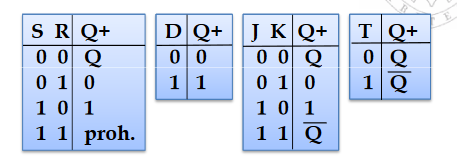
\includegraphics[width = 0.4\textwidth]{images/Tema_4/Tabla_Verdad_Biiestables.PNG}
		\caption{Tabla de verdad de los distintos tipos de biestables}
	\end{figure}
	\vfill
	\null
	\begin{figure}[H]
		\centering
		\includegraphics[width = 0.4\textwidth]{images/Tema_4/Ecuaciones_Características_Biestables.PNG}
		\caption{Ecuaciones características de los distintos tipos de biestables}
	\end{figure}
\end{multicols}
\newpage
\subsection{Biestables asíncronos: Latch}
La salida cambia cuando cambian las entradas:
\begin{figure}[H]
	\centering
	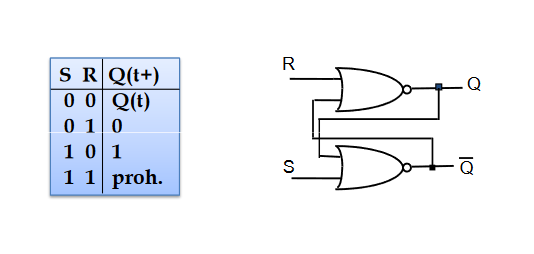
\includegraphics[width=0.8\textwidth]{images/Tema_4/Ejemplo_Latch.PNG}
	\caption{Ejemplo Latch S-R}
\end{figure}
\subsection{Biestable síncrono sensible a nivel: Latch síncrono}
La salida cambia cuando está activa la señal de capacitación (enable)
\begin{figure}[H]
	\centering
	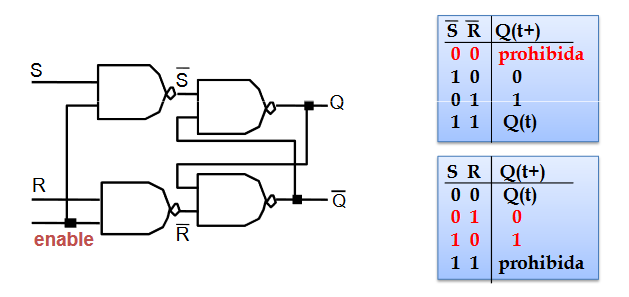
\includegraphics[width=0.8\textwidth]{images/Tema_4/Ejemplo_Latch_Sincrono.PNG}
	\caption{Ejemplo Latch síncrono S-R}
\end{figure}

Para que este biestable sea un tipo D, debemos cambiar el enable para que sea un clk
\begin{figure}[H]
	\centering
	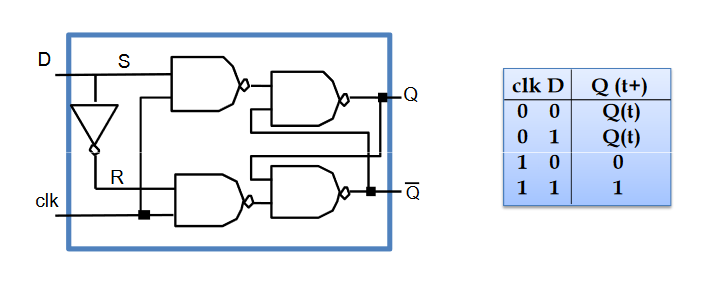
\includegraphics[width=0.8\textwidth]{images/Tema_4/Ejemplo_Latch_D.PNG}
	\caption{Ejemplo Latch tipo D}
\end{figure}

\subsection{Problemas}
Si utilizamos latches debemos garantizar que el pulso de reloj sea más corto que el retardo del latch y que las entradas se mantienen constantes durante el pulso del reloj.

Una alternativa es usar Flip-Flops, que son más fiables. Son disparados por flanco: la salida sólo varía durante la transición del reloj(que es una entrada dinámica).

\subsection{Flip-Flop disparado por flanco}
\begin{multicols}{2}
	\begin{itemize}
		\item clk = 0
		      \begin{itemize}
			      \item R = 1 y S = 1 independientemente del valor de D
			      \item P1 = $\overline{D}$ y P2 = $\overline{P1}$ = D
		      \end{itemize}
		\item clk = 0 $\rightarrow$ 1
		      \begin{itemize}
			      \item S = $\overline{P2}$ = $\overline{D}$ y R = $\overline{P1}$ = D
		      \end{itemize}
		\item clk = 1
		      \begin{itemize}
			      \item Los cambios en D no afectan a R y S
		      \end{itemize}
	\end{itemize}
	\vfill
	\null
	\begin{figure}[H]
		\centering
		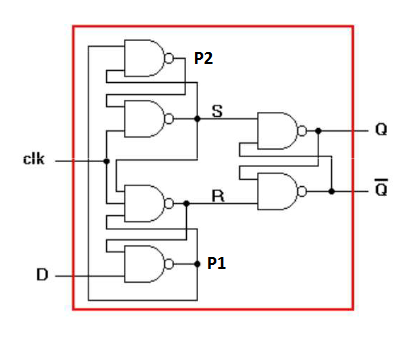
\includegraphics[width = 0.3\textwidth]{images/Tema_4/Flip_Flop_Flanco.PNG}
		\caption{Ejemplo Flip-Flop disparado por flanco}
	\end{figure}
\end{multicols}

\subsection{Biestable maestro-esclavo: FF}
Se lee la entrada en un nivel y se modifica la salida en el contrario:
\begin{figure}[H]
	\centering
	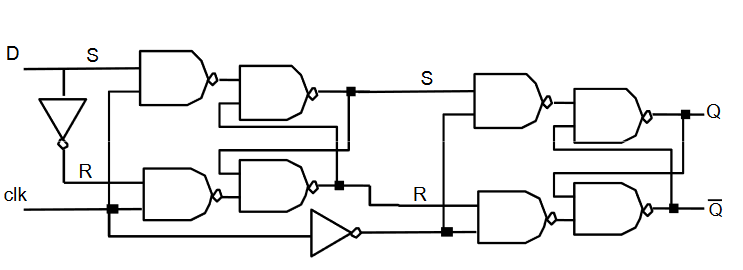
\includegraphics[width=0.8\textwidth]{images/Tema_4/Biestable_Maestro_Esclavo.PNG}
	\caption{Biestable Maestro-Esclavo}
\end{figure}

\subsection{Comparación del comportamiento temporal de los biestables}

\begin{table}[H]
	\centering
	\begin{tabularx}{\textwidth}{|X|X|X|}
		\hline
		\textbf{Tipo}                       & \textbf{?`Cuándo se muestrean las entradas?}                                                 & \textbf{?`Son válidas las entradas?}                    \\
		\hline
		\textbf{Latch sin reloj}            & siempre                                                                                      & retardo de propagación desde el cambio en la entrada    \\
		\hline
		\textbf{Latch sensible a nivel}     & reloj en alta ($T_{setup}$ y $T_{hold}$ a cada lado del eje de bajada)                       & retardo de propagación desde flanco de subida del reloj \\
		\hline
		\textbf{Flip-Flop flanco de subida} & transición de reloj de baja a alta  ($T_{setup}$ y $T_{hold}$ a cada lado del eje de subida) & retardo de propagación desde flanco de subida de reloj  \\
		\hline
		\textbf{Flip-Flop flanco de bajada} & transición de reloj de alta a baja ($T_{setup}$ y $T_{hold}$ a cada lado del eje de bajada)  & retardo de propagación desde flanco de bajada del reloj \\
		\hline
	\end{tabularx}
\end{table}

\subsection{Registros}
Hay de distintos tipos:
\begin{itemize}
	\item Según temporización:
	      \begin{itemize}
		      \item Disparado por nivel
		            \begin{figure}[H]
			            \centering
			            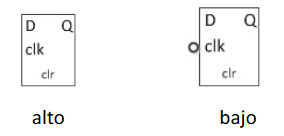
\includegraphics[width= 0.3\textwidth]{images/Tema_4/registros_nivel.PNG}
			            \caption{registros según nivel}
		            \end{figure}
		      \item Disparado por flanco
		            \begin{figure}[H]
			            \centering
			            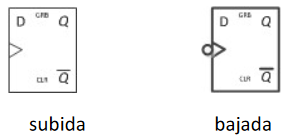
\includegraphics[width= 0.3\textwidth]{images/Tema_4/registros_flanco.PNG}
			            \caption{registros según nivel}
		            \end{figure}
	      \end{itemize}
	\item Según funcionalidad
	      \begin{itemize}
		      \item \gls{pipo}
		      \item \gls{sipo}
		      \item \gls{piso}
		      \item \gls{siso}
	      \end{itemize}
\end{itemize}

\section{Diseño Algorítmico}

El diseño algorítmico es una modo de especificación e implementación de sistemas digitales, que permite sistematizar y automatizar en gran medida su construcción. Parte siempre de una especificación en la que el comportamiento del sistema se describe en forma de un algoritmo (cómo calcular la salida en función de la entrada). Esto se implementa con una unidad de control y una ruta de datos.

Los sistemas algorítmicos son sistemas secuenciales síncronos. El comportamiento está definido implícitamente: no se especifica el valor de z si no el modo de calcularlo (el algoritmo).
\begin{figure}[H]
	\centering
	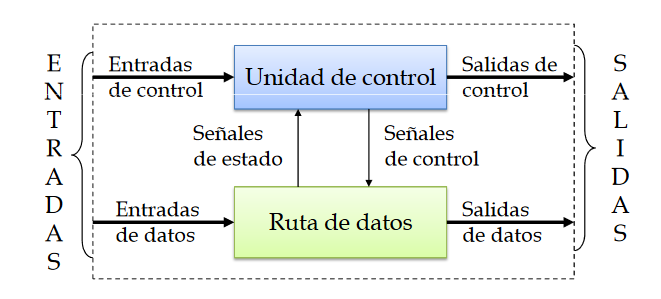
\includegraphics[width=0.7\textwidth]{images/Tema_4/Modelo_algoritmico.PNG}
	\caption{Modelo de sistema algorítmico}
\end{figure}

\subsection{Proceso de diseño: resumen}
Primero se define el sistema: se especifican las entradas, salidas, función y bloques disponibles.\\
Seguidamente se crea un diagrama \gls{asm}: obtenemos un conjunto ordenado y finito de operaciones y un modelo de máquina de estados generalizada.\\

Por último, diseñamos la unidad de control, la ruta de datos y las ensamblamos
\begin{enumerate}
	\item Estudio de la especificación:
	      \begin{itemize}
		      \item Esquema de pasos secuenciales a seguir (algoritmo)
		      \item Posible \gls{hw} a utilizar (módulos específicos completos)
	      \end{itemize}
	\item Creación de un diagrama \gls{asm} partiendo de las conclusiones del apartado 1, crear un diagrama que cumpla las especificaciones.
	\item Diseño de la unidad de control:
	      \begin{itemize}
		      \item Codificar cada uno de los estados del \gls{asm}
		      \item Codificar el cambio de estado
		            \begin{itemize}
			            \item Mediante señales internas de control
			            \item Mediante señales externas de control
		            \end{itemize}
		      \item Codificar las señales de control hacia la ruta de datos: cada estado tendrá asociados unos valores de todas las señales que controlan los módulos complejos
	      \end{itemize}
	\item Diseño de la ruta de datos:
	      \begin{itemize}
		      \item Interconectar las señales de control externas e internas a los módulos
		      \item Interconectar las señales de control (obtenidas en el apartado 3) a los módulos de la ruta de datos
	      \end{itemize}
\end{enumerate}


\subsection{Diagrama de Máquina de Estados Algorítmica (ASM)}
Esta es una forma gráfica de representar el algoritmo.
Los elementos de un diagrama son:
\begin{itemize}
	\item Cajas de estado: asignaciones y operaciones simultáneas.
	\item Cajas de decisión: bifurcación condicional con dos posibilidades.
	\item Cajas de salida condicional: asignaciones que se realizan cuando se cumple una condición.
	\item Bloque ASM: una caja de estado con red de cajas de decisión y de salida condicional.
\end{itemize}
